\documentclass[11pt]{article}
\usepackage[margin=1in]{geometry}
\usepackage{amsfonts,amsmath,amssymb}
\usepackage[none]{hyphenat}
\usepackage{fancyhdr}
\usepackage{graphicx}
\usepackage{float}
\usepackage{enumitem}
\usepackage{hyperref}
\usepackage[noline,boxed]{algorithm2e}
\usepackage[skins]{tcolorbox}
\usepackage[nottoc,notlot,notlof]{tocbibind}
\usepackage{xcolor}
\usepackage{mathtools}
\usepackage{physics}
\usepackage{minted}
% \usepackage{fourier}

% add these two lines to your long preamble    
% \DeclareMathAlphabet{\mathcal}{OMS}{cmsy}{m}{n}
% \SetMathAlphabet{\mathcal}{bold}{OMS}{cmsy}{b}{n}

% \usemintedstyle{borland}

%\parindent 0ex
\setlength{\parindent}{4em}
\setlength{\parskip}{0em}
\renewcommand{\baselinestretch}{1.5}
\graphicspath{images/}
\begin{document}

\begin{titlepage}
\begin{center}
\vspace*{0.5cm}
\Large{\textbf{SM 402: Basic Computational Topology}}\\
\Large{\textbf{Implementation Project}}\\
\vfill
% \line(1,0){400}\\[1mm]
% \vspace{10mm}
% {\textbf{Experiment 2: Experiments with simple and double pendulums}}
% \vspace{10mm}
% \line(1,0){400}\\[1mm]
\vfill
By \\ 
IMT2020042 Gousepeer Arella \\
IMT2020085 Harshadeep Donapati \\
IMT2020082 Prudhvi Nath Reddy \\
IMT2020522 Prasanth Reddy Lomada \\
\end{center}
\end{titlepage}

\tableofcontents
\thispagestyle{empty}
\clearpage
\setcounter{page}{1}

\section{Problem Statement}
Problem Number : 4 \\
Given any input simplicial complex (up to 3 -dimensional), compute $\beta_3$ 
using the boundary matrix method.

\section{Algorithm}
Formula used to calculate $\beta_3$: \\
\begin{equation}
    \beta_3 = dim(Ker(\partial_3)) - dim(Im(\partial_4))
\end{equation}
In our python file, we take the filename (.gts file) as an input from the user and process the file. \\
We know that $\partial_3$ and $\partial_4$ are defined as:
\begin{equation*}
    \partial_3 : C_{3}(K) \to C_{2}(K) 
\end{equation*}
\begin{equation*}
    \partial_4 : C_{4}(K) \to C_{3}(K)
\end{equation*}
$\partial_k$ boundary matrix row labels are basis for $C_{k-1}(X)$ and column labels are the basis for $C_{k}(X)$.  \\
Kernel of a matrix is nullspace of the matrix and image is columnspace of a matrix.

\section{Steps to run the code}
Make sure you have \ttfamily \texttt{python3 and numpy and plotly} \normalfont installed. 
Use the command \ttfamily \texttt{pip3 install numpy plotly}  \normalfont to install them. \\
For best results for tetrahedron, use \ttfamily \texttt{tetra.py}.\normalfont Use \ttfamily \texttt{Tetrahedron.gts} \normalfont as your input file. \\
For Torus and TangleCube, use the command \ttfamily \texttt{python3 only.py} \normalfont to run it. Then enter the name of the of the \ttfamily \texttt{.gts} \normalfont file.

\usemintedstyle{vs}
\section{Code}
\href{https://github.com/harsha-deep/BCTImplementationProject/blob/main/only.py}{\textbf{only.py}}
\begin{minted}{python}
import time
import numpy as np
import os
import plotly.graph_objects as go

begin = time.time()


def convert_float(nested):
    return [[float(x) for x in lst] for lst in nested]


def convert_int(nested):
    return [[int(x) for x in lst] for lst in nested]


def open_file(file_name):
    try:
        with open(file_name, 'r') as f:
            line = f.readline()
            lst = line.split(' ')
            no_vertices = int(lst[0])
            no_edges = int(lst[1])
            no_faces = int(lst[2])
            print("Number of vertices:", no_vertices)
            print("Number of edges:", no_edges)
            print("Number of faces:", no_faces)

            vertices = []
            edges = []
            faces = []

            for i in range(no_vertices):
                line = f.readline()
                vertices.append(list(line.replace('\n', '').split(' ')))

            for i in range(no_edges):
                line = f.readline()
                edges.append(list(line.replace('\n', '').split(' ')))

            for i in range(no_faces):
                line = f.readline()
                faces.append(list(line.replace('\n', '').split(' ')))

    except OSError as e:
        print(e.strerror)

    print("vertices:", convert_float(vertices))
    print("edges:", convert_int(edges))
    print("faces:", convert_int(faces))

    try:
        os.mknod('vertices.txt')

    except FileExistsError as e:
        print(e.strerror)

    with open("vertices.txt", "a") as f:
        for lst in vertices:
            f.write(lst[0] + ' '+lst[1] + ' ' + lst[2] + '\n')

    pts = np.loadtxt(np.DataSource().open(
        'vertices.txt'))

    x, y, z = pts.T

    fig = go.Figure(
        data=[go.Mesh3d(x=x, y=y, z=z, color='cyan', opacity=0.5)])

    fig.show()

    os.remove('vertices.txt')


if __name__ == '__main__':
    file_name = input("Enter the name of the file: ")
    open_file(file_name)
    end = time.time()
    print("Time elapsed:", end - begin, 's')

\end{minted}

\subsection{Github Link} \\
You can also visit the below link. \\
\url{https://github.com/harsha-deep/BCTImplementationProject}

\section{Note}
The code is not complete. We are unable to calculate $\partial_3$ and $\partial_4$.

\section{Screenshots}
% \begin{figure}[h]
% \centering
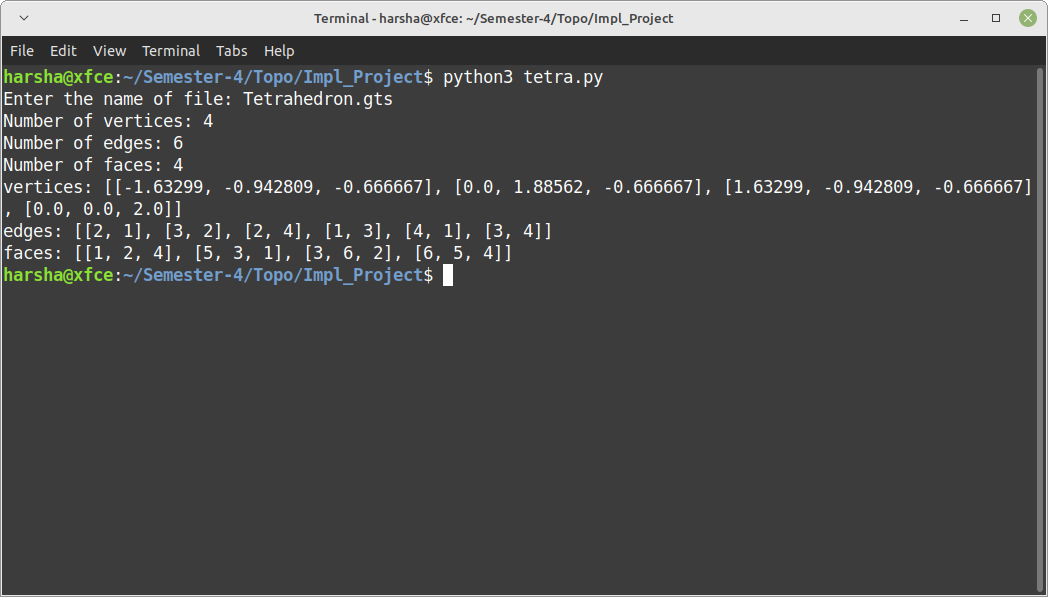
\includegraphics[scale=0.45]{img/tetrahedron_results.png} \\
\includegraphics[scale=0.5]{img/newplot.png}
Tetrahedron. \\
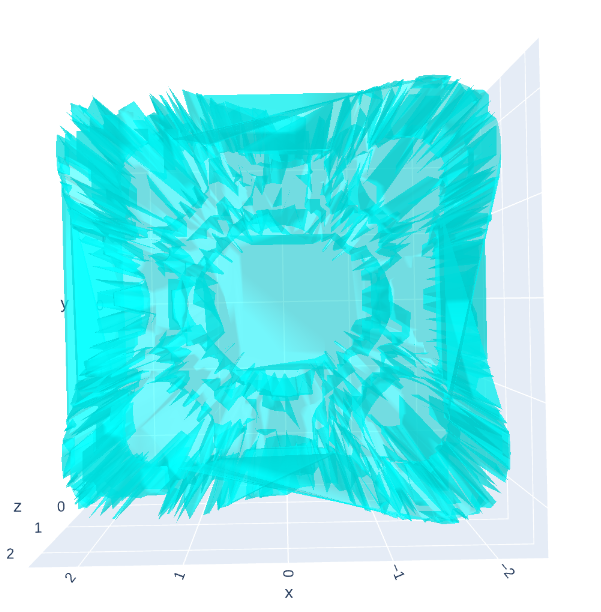
\includegraphics[scale=0.5]{img/tangle.png}
Tangle cube. \\
% \caption{Figure of tetrahedron generated.}
% \label{fig:stack}
% \end{figure}

\section{References}
1 . \url{https://en.wikipedia.org/wiki/Simplicial_complex} \\
2. \url{https://jeremykun.com/2013/04/10/computing-homology/} \\
3. \url{https://jeremykun.com/2014/01/23/fixing-bugs-in-computing-homology/} \\
4. \url{http://gts.sourceforge.net/samples.html} \\
5. \url{https://plotly.com/python/3d-mesh/}

\end{document}


